\documentclass[border=3mm]{standalone}
\usepackage{tikz}
\usetikzlibrary{positioning,fit,arrows.meta,backgrounds}

\tikzset{
    module/.style={%
        draw, rounded corners,
        minimum width=#1,
        minimum height=7mm,
        font=\sffamily
        },
    module/.default=2cm,
    >=LaTeX
}

\begin{document}
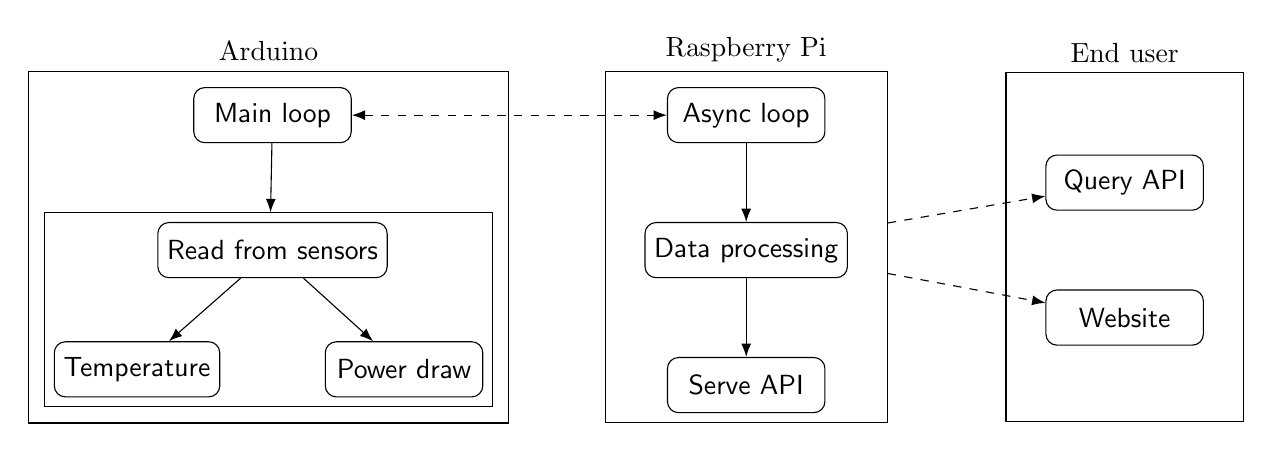
\begin{tikzpicture}
    \node[module] (Loop) {Main loop};
    \node[module, below=of Loop] (Read) {Read from sensors};
    \node[module, below left=8mm and -8mm of Read] (Temp) {Temperature};
    \node[module, below right=8mm and -8mm of Read] (Power) {Power draw};
    \node[fit=(Read) (Temp) (Power), draw] (SensorBox) {};
    \node[fit=(SensorBox) (Loop), draw, inner sep=2mm, label={Arduino}] (ArduinoBox) {};
    \draw[->] (Read)--(Temp);
    \draw[->] (Read)--(Power);
    \draw[->] (Loop)--(SensorBox);

    \node[module, right=2cm of {Loop-|ArduinoBox.east}] (AsyncLoop) {Async loop};
    \node[module, below=of AsyncLoop] (Data) {Data processing};
    \node[module, below=of Data] (PiAPI) {Serve API};
    \node[fit={(Data) (Data|-ArduinoBox.south) (Data|-ArduinoBox.north)},
          draw, inner xsep=5mm,
          inner ysep=-\pgflinewidth, label={Raspberry Pi}]
          (PiBox) {};
    \draw[->] (AsyncLoop)--(Data);
    \draw[->] (Data)--(PiAPI);

    \node[module, above right=5mm and 2cm of {Data-|PiBox.east}] (API) {Query API};
    \node[module, below=of API] (Web) {Website};
    \node[fit={(Web) (Web|-PiBox.south) (Web|-PiBox.north)},
          draw, inner xsep=5mm,
          inner ysep=-\pgflinewidth, label={End user}]
          (User) {};

   \draw[<->,dashed] (Loop)--(AsyncLoop);
   \draw[->,dashed] (PiBox)--(API);
   \draw[->,dashed] (PiBox)--(Web);
\end{tikzpicture}
\end{document}
%%% Local Variables:
%%% mode: latex
%%% TeX-master: t
%%% End:
